\documentclass[a4paper,12pt]{article}
\usepackage[english]{babel}
\usepackage{graphicx}
\usepackage{csvsimple}
\usepackage{pgfplotstable}
\usepackage{booktabs}
\usepackage{chngcntr}
\usepackage{sectsty}
\usepackage{pdfpages}
\usepackage{longtable}
\usepackage{tocloft}

%\usepackage[pdftex]{graphicx}
\usepackage[ansinew]{inputenc}
\usepackage{geometry}
%\usepackage{bbold}
\geometry{a4paper,left=2.5cm,right=2.5cm, top=2.5cm, bottom=3cm}
\newcommand{\HRule}{\rule{\linewidth}{0.5mm}}

\usepackage{textcomp}
\usepackage[hyphens,spaces]{url}

\begin{document}
\sloppy
\sectionfont{\LARGE}
\subsectionfont{\Large}
\subsubsectionfont{\Large}
\counterwithin{figure}{section}
\counterwithin{table}{section}

\begin{titlepage}


%%LR
\sffamily

\begin{center}


% Oberer Teil der Titelseite:

\includegraphics[width=0.3\textwidth]{../figures/LMU-logo.jpg}
\hfill

\includegraphics[width=0.4\textwidth]{../figures/TUM-logo.jpg}  
\\[5cm]

{\LARGE Department of Bioinformatics and Computational Biology}\\[0.5cm]
{Technische Universit\"at M\"unchen}\\
[2cm]
{\Large Master's Thesis in Bioinformatics}\\[1.5cm]

% Title
\HRule \\[0.4cm]
{ \huge \bfseries Variation of HERV elements in the KORA cohort
}\\[0.4cm]

\HRule \\[1.5cm]

{\Large Julian Schmidt}\\[2.5cm]

\vfill
\end{center}
\end{titlepage}
\pagestyle{empty}

%%LR comprehensive title
\begin{titlepage}
{\sffamily


\begin{center}

\includegraphics[width=0.3\textwidth]{../figures/LMU-logo.jpg}
\hfill

\includegraphics[width=0.4\textwidth]{../figures/TUM-logo.jpg}  
\\[1.5cm]  

{\LARGE Department of Bioinformatics and Computational Biology}\\[0.5cm]
{Technische Universit\"at M\"unchen}\\[1cm]

{\Large Master's Thesis in Bioinformatics}\\[2cm]
{\textbf{\LARGE Variation of HERV elements in the KORA cohort}}\\[2cm]
{\textbf{\LARGE Variation von HERV elementen in der KORA Kohorte}}\\[4cm]

\end{center}
\begin{center}\Large
  \begin{tabular}{ll}
    Author:& Julian Schmidt\\
    Supervisor: & Dr. Matthias Heinig\\
    Advisor:        & Johann Hawe\\
    Submitted:     &  15.03.2018\\
  \end{tabular}
\end{center}

}% end title page

\end{titlepage}

\pagenumbering{gobble}

\tableofcontents
\newpage

\pagestyle{plain}
\pagenumbering{arabic}
\section{Introduction}

\subsection{Regulation of cell functions and Epigenetics}
\begin{itemize}
\item central dogma of biology
\item rising importance of other factors atop DNA \textrightarrow epigenetics
\item quick overview epigenetic marks
\item chromatin states
\item DNA methylation 
\item snp -> cpg -> expression pattern
\item TF <-> cpg interaction
\end{itemize}


\subsection{Human endogenous retroviruses}
\begin{itemize}
\item first humane genome -> "junk DNA"
\item ongoing discovery for non-coding regions
\item still masking of difficult sequence for many analysis -> repeats
\item repeat classes -> ... -> herv
\item herv origin - ...-virus like 
\item herv structure: LTR - pol - env - ... - LTR
\item discovered roles of hervs in general regulation/diseases
\item 
\end{itemize}

\subsection{Effect network analysis}
\begin{itemize}
\item many bioinformatics methods find correlations, but not direct cause
\item attempt to discern direct connections from bigger data webs
\item hope to find possible biological mechanisms of gene regulation = path in model
\item used approach: Gaussian Graphical models
\end{itemize}


\newpage
\section{Data}


\subsection{hERV annotation}
hERV annotation was pertained from RepeatMasker human annotation downloaded from the UCSC genome browser download section \url{(http://hgdownload.soe.ucsc.edu/goldenPath/hg19/database/rmsk.txt.gz)}.
 
The annotation then was filtered for elements containing "ERV" in the repeat name column. This lead to a total of 42508 elements with a mean width of 796 bp covering a total of 33.9 MB. This set will be called "hERV set 1", or short hERV s1.

Alternatively filtering the annotation for "ERV" in the superfamily column leads to 696689 elements. They have a mean width of 379 bp and cover 263.7 MB. (hERV set 2/hERV s2)

A third set "hERV set 3" (hERV s3) was constructed by filtering the repeat name column for "hERV", which resulted in 21361 elements. 

\subsection{KORA}
The Expression, Methylation and Genotype data used in this work were generated by the platform for Cooperative Health Research in the Region of Augsburg - short KORA. It contains health surveys as well as examinations of individuals of German nationality living in the area of Augsburg, Bavaria.
The objective of KORA is to track changes in health conditions over a long period in order to identify and examine the causes, effects and development of chronical diseases.

The data comes from the Survey F4, which was conducted from 2006 to 2008 and comprised samples of 3080 individuals. F4 is a follow up study to the survey S4 performed from 1999 to 2001 and containing 4261 individuals. 

All measurements were performed on whole blood samples. Houseman blood counts\cite{} describing the composition of different cell types for each individual are available.

Not all essays are available for all samples. Therefore different analyses were performed on varying sets of indiviudals according to availability of the required data types.

\subsubsection{Expression}
The expression data was generated using the HumanHT-12 v3.0 Gene Expression BeadChip. The chip can measure expression values for 49576 probes. However only 47864 probes represent an actual genomic location. 

Measurements for 993 individuals are available from the KORA F4 survey. The comprise values for a total of 48803 probes per sample. Probes that do not map to a genomic location were excluded in all analyses, leaving 47864 probes. Of these 29521 are annotated to total of 19288 genes. 

To not lose information, especially in hERV regions that are usuallly sparesly annotated with genes, probes without genes were not discarded and most analyses were performed on probe level or only partially abstracting to gene level. 

\begin{figure}[tb]
	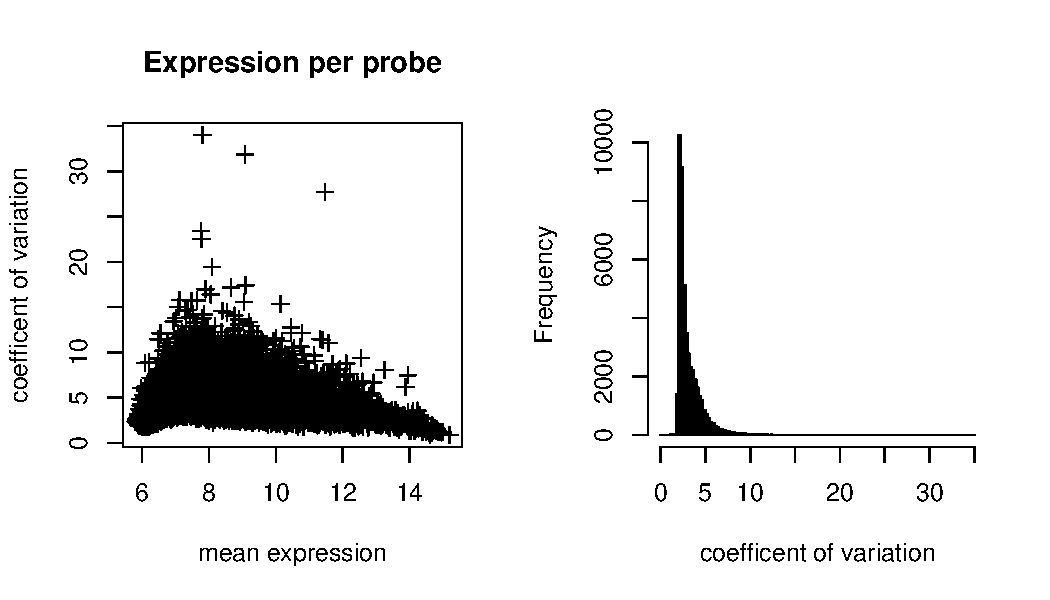
\includegraphics[scale = 1, keepaspectratio = true]{../figures/expr_var}  
	\caption{Coefficient of expression variance over 993 individuals}
    \label{fig:expr.var}
\end{figure}

\subsubsection{Methylation}
DNA methylation was measured using the Infinium HumanMethylation450K BeadChip, which interrogates methylation levels at 485577 genomic locations.  

Methylation data was available for 1727 individuals and 485512 sites, which make up all 'cg' and 'ch' probe type probes.
 
\subsubsection{Genotypes}
Genotyping was performed with the Affymetrix Axiom array. The Iluminus calling algorithm was used for genotype calling and missing values were imputed using the IMPUTE2 software\cite{10.1371/journal.pgen.1000529}. SNPs were filtered at IMPUTE value of 0.4. 

After excluding all SNPs with a minor allele frequency of less than one percent measurements of 9533127 SNPs for 3788 individuals were available. 

\subsubsection{Covariates}
Several covariates were known for each sample. These were age, sex, body mass index (BMI) and wide blood cell count, as well as experimental factors like storage time and RNA integrity number (RIN).

\subsubsection{Methylation quantitative trait loci}
Previously process methylation quantitative trait loci (meQTL) data was used. The data set contained a total of xxxxxx significantly associated cpg-snp pairs. 
xxxx distinct cpg-sites and xxxxxx snps were part of at least one meQTL. xxxx pairs consisted of cpgs and snps on the same chromosome, while xxxxx association were between different chromosomes. 

\subsection{Transcription factor binding}
Transcription factor binding sites were obtained from two publicy available sources: 

First was the third version of the track "Transcription Factor ChIP-seq (161 factors) from ENCODE with Factorbook Motifs"\cite{10.1101/gr.139105.112} downloaded from the UCSC genome browser download section (\url{http://hgdownload.cse.ucsc.edu/goldenPath/hg19/encodeDCC/wgEncodeRegTfbsClustered/wgEncodeRegTfbsClusteredWithCellsV3.bed.gz}).

It combines 690 high quality ENCODE ChIP-seq data sets, which were processed with the Factorbook motif discovery and annotation pipeline\cite{10.1101/gr.139105.112}. The pipeline uses the tools MEME-ChIP\cite{10.1093/bioinformatics/btr189} and FIMO\cite{10.1093/bioinformatics/btr064} from the MEME software suite and merges discovered motifs with known motifs from Jaspar\cite{10.1093/nar/gkx1126} and TransFac\cite{10.1093/nar/gkj143} using machine learning methods and manual curation. 

The track contains a total of 438044 distinct peaks for 161 transcription factors in 91 cell types. For our analyses we filtered and combined the peaks for 23 blood related cell types. This leaves a total of 2173371 peaks for 125 transcription factors.  

The second source was the ReMap project\cite{10.1093/nar/gku1280}. It combines 395 publicy available ChIP-seq data sets covering 132 different transcription factors across 83 cell lines. ReMap uses Bowtie2\cite{} to map reads to the human genome and the tool MACS\cite{} for peak calling. The finished data set was downloaded from the ReMap website\url{(http://tagc.univ-mrs.fr/remap/download/All/filPeaks_public.bed.gz)}.

It contains xxxxx peaks. After filtering for 19 blood related cell types a of xxxx peaks of xxx different transcription factors remained. 

Combining both filtered data sets lead to a total of xxxxx peaks of xxx transcription factors.


\subsection{Chromatin states}
Chromatin state annotations were downloaded from Roadmap Epgenomics Core 15-state model\url{http://egg2.wustl.edu/roadmap/data/byFileType/chromhmmSegmentations/ChmmModels/coreMarks/jointModel/final}. The Model provides a whole genome chromatin state annotation of 200 bp wide windows to the following 15 states: Active Transcription Start Site (TSS), Flanking Active TSS, Transcription at gene 5' and 4', Strong transcription, Weak transcription, Genic enhancers, Enhancers, ZNF genes \& repeats, Heterochromatin, Bivalent/Poised TSS, Flanking Bivalent TSS/Enhancer, Bivalent Enhancer, Repressed PolyComb, Weak Repressed PolyComb and Quiescent/Low. The model is available for 127 diverse cell lines. 

It was generated using ChromHMM v1.10\cite{10.1038/nmeth.1906} on the chromatin marks H3K4me1, H3K4me3, H3K27me3, H3K9me3, and H3K36me3. ChromHMM is based on a multivarate Hidden Markov Model. 

In this work the annotations for 27 blood related cell lines were used. To get the distribution of states for a single feature or a set of features the different annotations for the different cell lines were weighted according to the houseman counts and summed up.

\section{Methods}
\subsection{Overlaps}
The task of whether HERV elements contained any annotated elements like expression probes, genes, cpg sites and transcription factor binding sites (tfbs) was performed using funtion "findOverlaps" from the Bioconductor package "GenomicRanges"\cite{10.1371/journal.pcbi.1003118}. 

Features were considered to be of interest for the analysis of an HERV element, if they overlapped by at least one base pair.

 were also generated for the herv elements plus 1kb and 2kb flanking regions. 

\subsection{Data normalization}


\begin{itemize}
\item calculate residuals with linear regression to select covariates
\item expression: 
\item methylation:
\end{itemize}
\subsection{eQTL/eQTM calculation}
\begin{itemize}
\item R package MatrixEQTL
\item determines correlation between snp and expression values by linear regression model
\item reduction to simple matrix multiplications
\begin{itemize}
\item mean -> 0
\item variance -> 0-1
\item allows fast calculation
\end{itemize}
\item paramters: 
\begin{itemize}
\item model: linear
\item thresholds: cis = 10e-6, trans 10e-8
\item cis-dist: 5e5
\end{itemize}
\end{itemize}
\subsection{Functional Analysis of Gene Sets}
\begin{itemize}
\item packages GSEABase, GOstats
\item generate GeneSetCollection for Gene Symbol -> GO term, for all pairs with evidence
\item test vor overrepresentation of terms in set of genes against background set using Hypergeometric test (hyperGTest)
\end{itemize}
\subsection{Gaussian Graphical Models}
\begin{itemize}
\item I'm fucking afraid of writing this part...
\end{itemize}

\newpage
\section{Results}
\subsection{Normalized Data}
\begin{itemize}
\item raw var vs residual var
\item 
\end{itemize}
\subsection{HERV region features}
\subsubsection{Expression}
Using hERV set 1 there are a total of 191 overlaps of at least 1 bp between a hERV element and a region measured in the expression array. 174 hERV elements overlap with 188 different expression probes. 

The expression probes have 1338 overlaps with the annotated elements in hERV set 2. 1274 hERV elements overlap with 1317 different expression probes.

The coefficents of variance for the expression probes that overlap with the hERV sets are shown in Figure \ref{fig:herv.expr.var}

When inspecting not only direct overlaps, but the region of +/- 1kb around the hERV elements, there are 517 overlaps (476 hERV elements, 349 probes) for set 1 and 6812 overlaps (6336 hERV elements, 4712 probes) for set 2.

Enlarging the flanking regions to 2kb leads to 973 (870 hERV elements, 548 probes) and 13398 (12201 hERV elements, 8044 probes) overlaps for set 1/2 respectively.



\subsubsection{Methylation}
Using hERV set 1 there are a total of 1602 overlaps of hERV elements and measured methylation sites. 1021 hERV elements overlap with 1595 different methylation sites.

hERV set 2 has 17162 overlaps. These are constituted by 13141 hERV elements and 17137 methylation sites.

Including the 1kb flanking regions of the hERV elements leads to 6785 overlaps (3470 hERV elements, 4497 methylation probes) for set 1 and 119763 overlaps (66249 hERV elements, 78501 methylation probes) for set 2.

With a flanking region of 2k this increases to 13559 overlaps (5645 hERV elements, 7792 methylation probes) for set 1 and 259739 overlaps (110524 hERV elements, 139036 methylation probes) for set 2. 

\subsubsection{Genotypes}
Measurements for a total of 80754 SNPs within hERV set 1, that occurr in at least  sample, are available.

\subsubsection{Chromatin states}

\subsection{eQTLs}

\subsection{eQTMs}

\subsection{hERV realated regulatory networks}

\newpage
\section{Discussion}

\newpage
\section{Conclusion}

\newpage
\bibliography{mybib}{}
\bibliographystyle{unsrt}

\end{document}